\setchapterstyle{kao}
\setchapterpreamble[u]{\margintoc}

\setchapterstyle{kao}
\setchapterpreamble[u]{\margintoc}
\chapter{Results}


In this chapter. Prediction model results will be discussed. An quantitative comparison to other models is provided.

To evaulate the quality of the model and its potential benefits.

\section{Quantitative comparison to other models}
\label{sec:res-comparison}

% Please add the following required packages to your document preamble:

\begin{table*}[h!]
    \caption{Comparison of model performance metrics including Mean Absolute Error (MAE) and Mean Squared Error (MSE) with their normalized and power variants.}
    \label{tab:my-table}
    \begin{tabular}{p{3.3cm} p{1.5cm} p{1.8cm} p{2.2cm} p{1.5cm} p{1.8cm} p{2.2cm}}
        \toprule
        \textbf{Model}         & \textbf{MAE} & \textbf{MAE norm} & \textbf{MAE power} & \textbf{MSE} & \textbf{MSE norm} & \textbf{MSE power} \\
        \midrule
        ChargingProfileModel   & 86.3404      & 0.0447            & 1553.9763          & 33729.4410   & 0.0057            & 7748441.2767       \\
        LinearRegression       & 107.9335     & 0.0962            & 2181.7242          & 41590.8896   & 2.9124            & 10658337.9148      \\
        TrainAverageModel      & 87.9659      & 0.0435            & 1629.9461          & 33973.4273   & 0.0057            & 7853195.2634       \\
        ValidationAverageModel & 87.9659      & 0.0435            & 1629.9461          & 33973.4273   & 0.0057            & 7853195.2634       \\
        XGBoost                & 92.4132      & 0.0456            & 1639.3703          & 42282.8242   & 0.0065            & 7993035.6818       \\
        \bottomrule
    \end{tabular}
\end{table*}
\section{Qualitative latent profiles analysis}

\textit{Inspection of the outputed latent profiles in prague together with hypotethising if that at least makes sense. Show the latent profile contribution on the training dataset because it interesting to see what it learned from the data and not necesarily rating its prediction power.}

\section{Tool for visualisation of prediction results}
To be able to inspect the prediction results in spatial context a tool was also developed with use of Streamlit\sidecite{StreamlitFasterWay2021}. The dashboard is in a form of a webapplication.
It consists of two screens.
First one allows inspection of overall model losses as visible in \ref{sec:res-comparison}. In bar charts and tabular formats. Where the bar chart shows all the types of losses relatively to each other.
\begin{figure}
    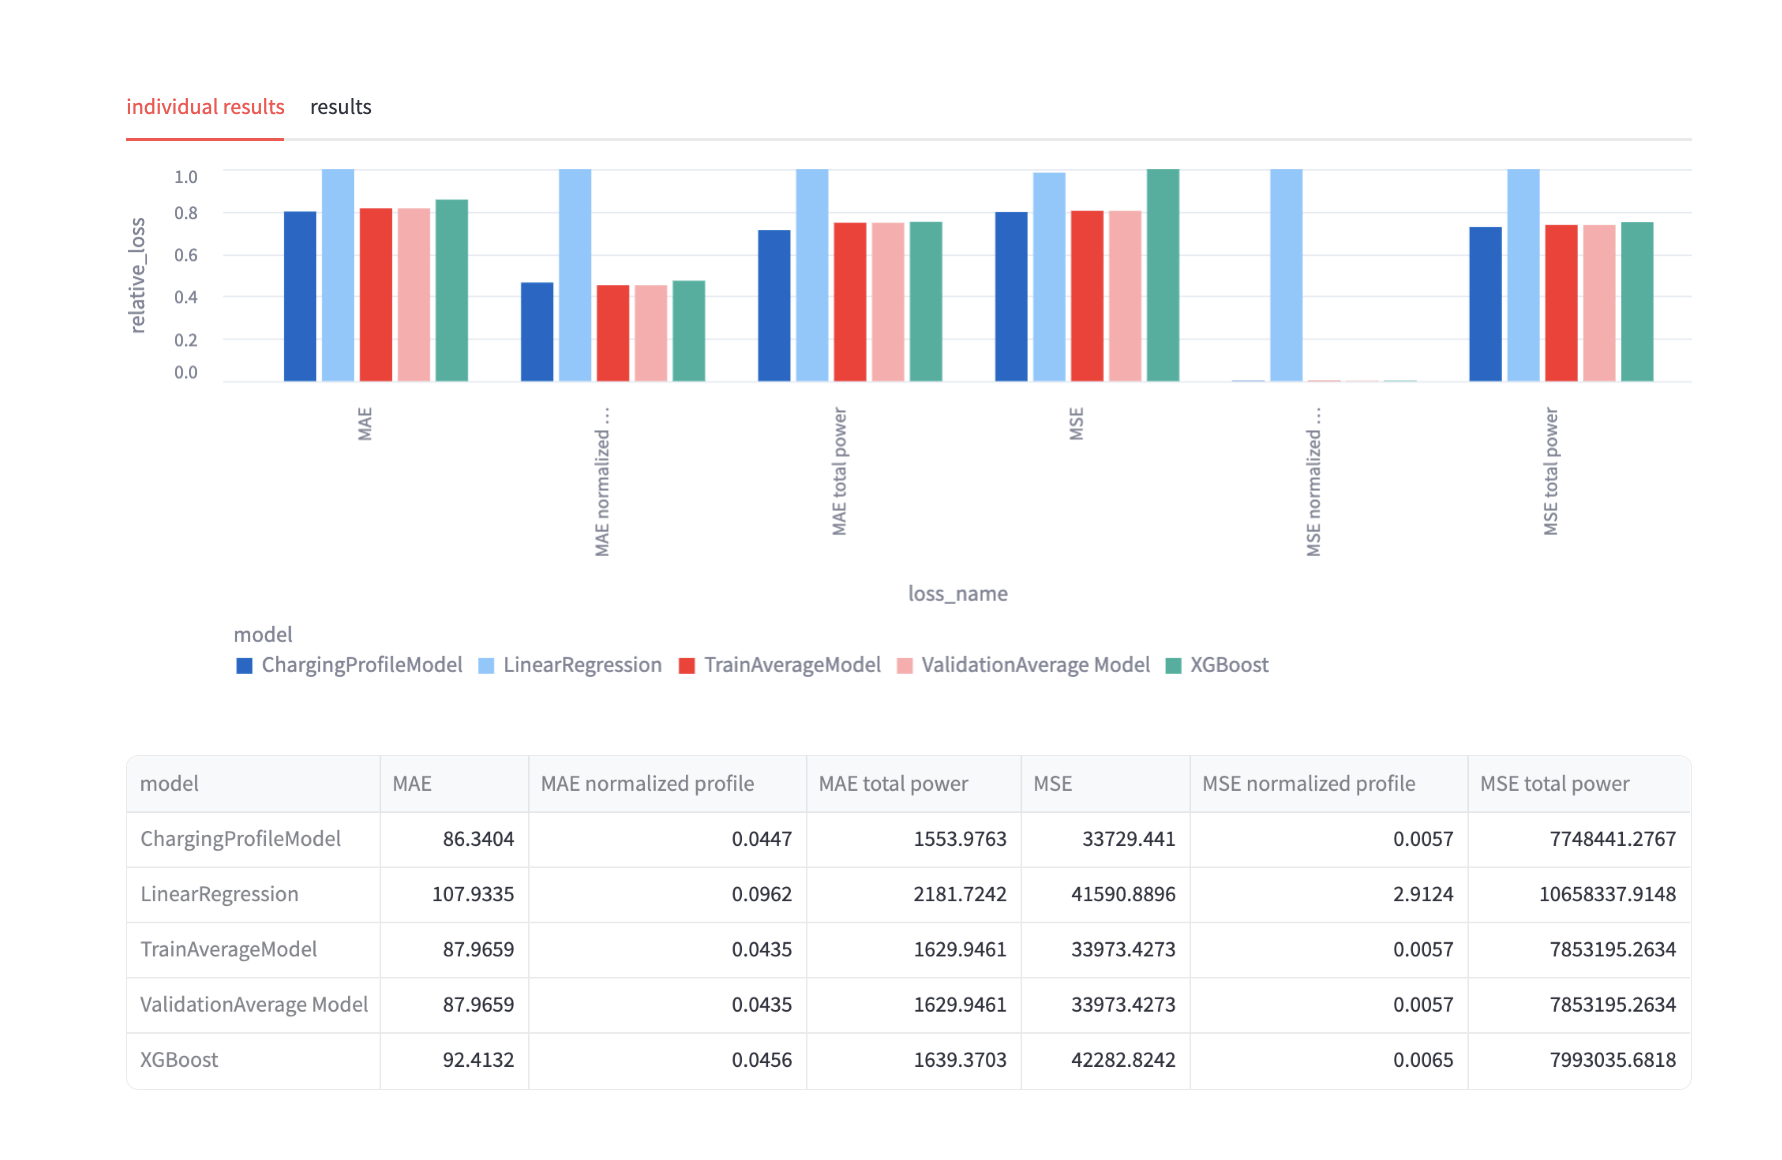
\includegraphics{data-dashboard-losses.png}
    \caption[]{Data dashboard website showing bar chart with relative losses of the models}
    \labfig{dasboard-all}
\end{figure}

The second screen displays table of all charging location together with day of the week and month. The individual rows of the table are selectable. When selection haapens location of the charger in map is shown and prediction from the model together with other models used for comparison is computed and its results are shown in a bar chart graph. Together with losses agains the original label $y$ value.

\begin{figure}
    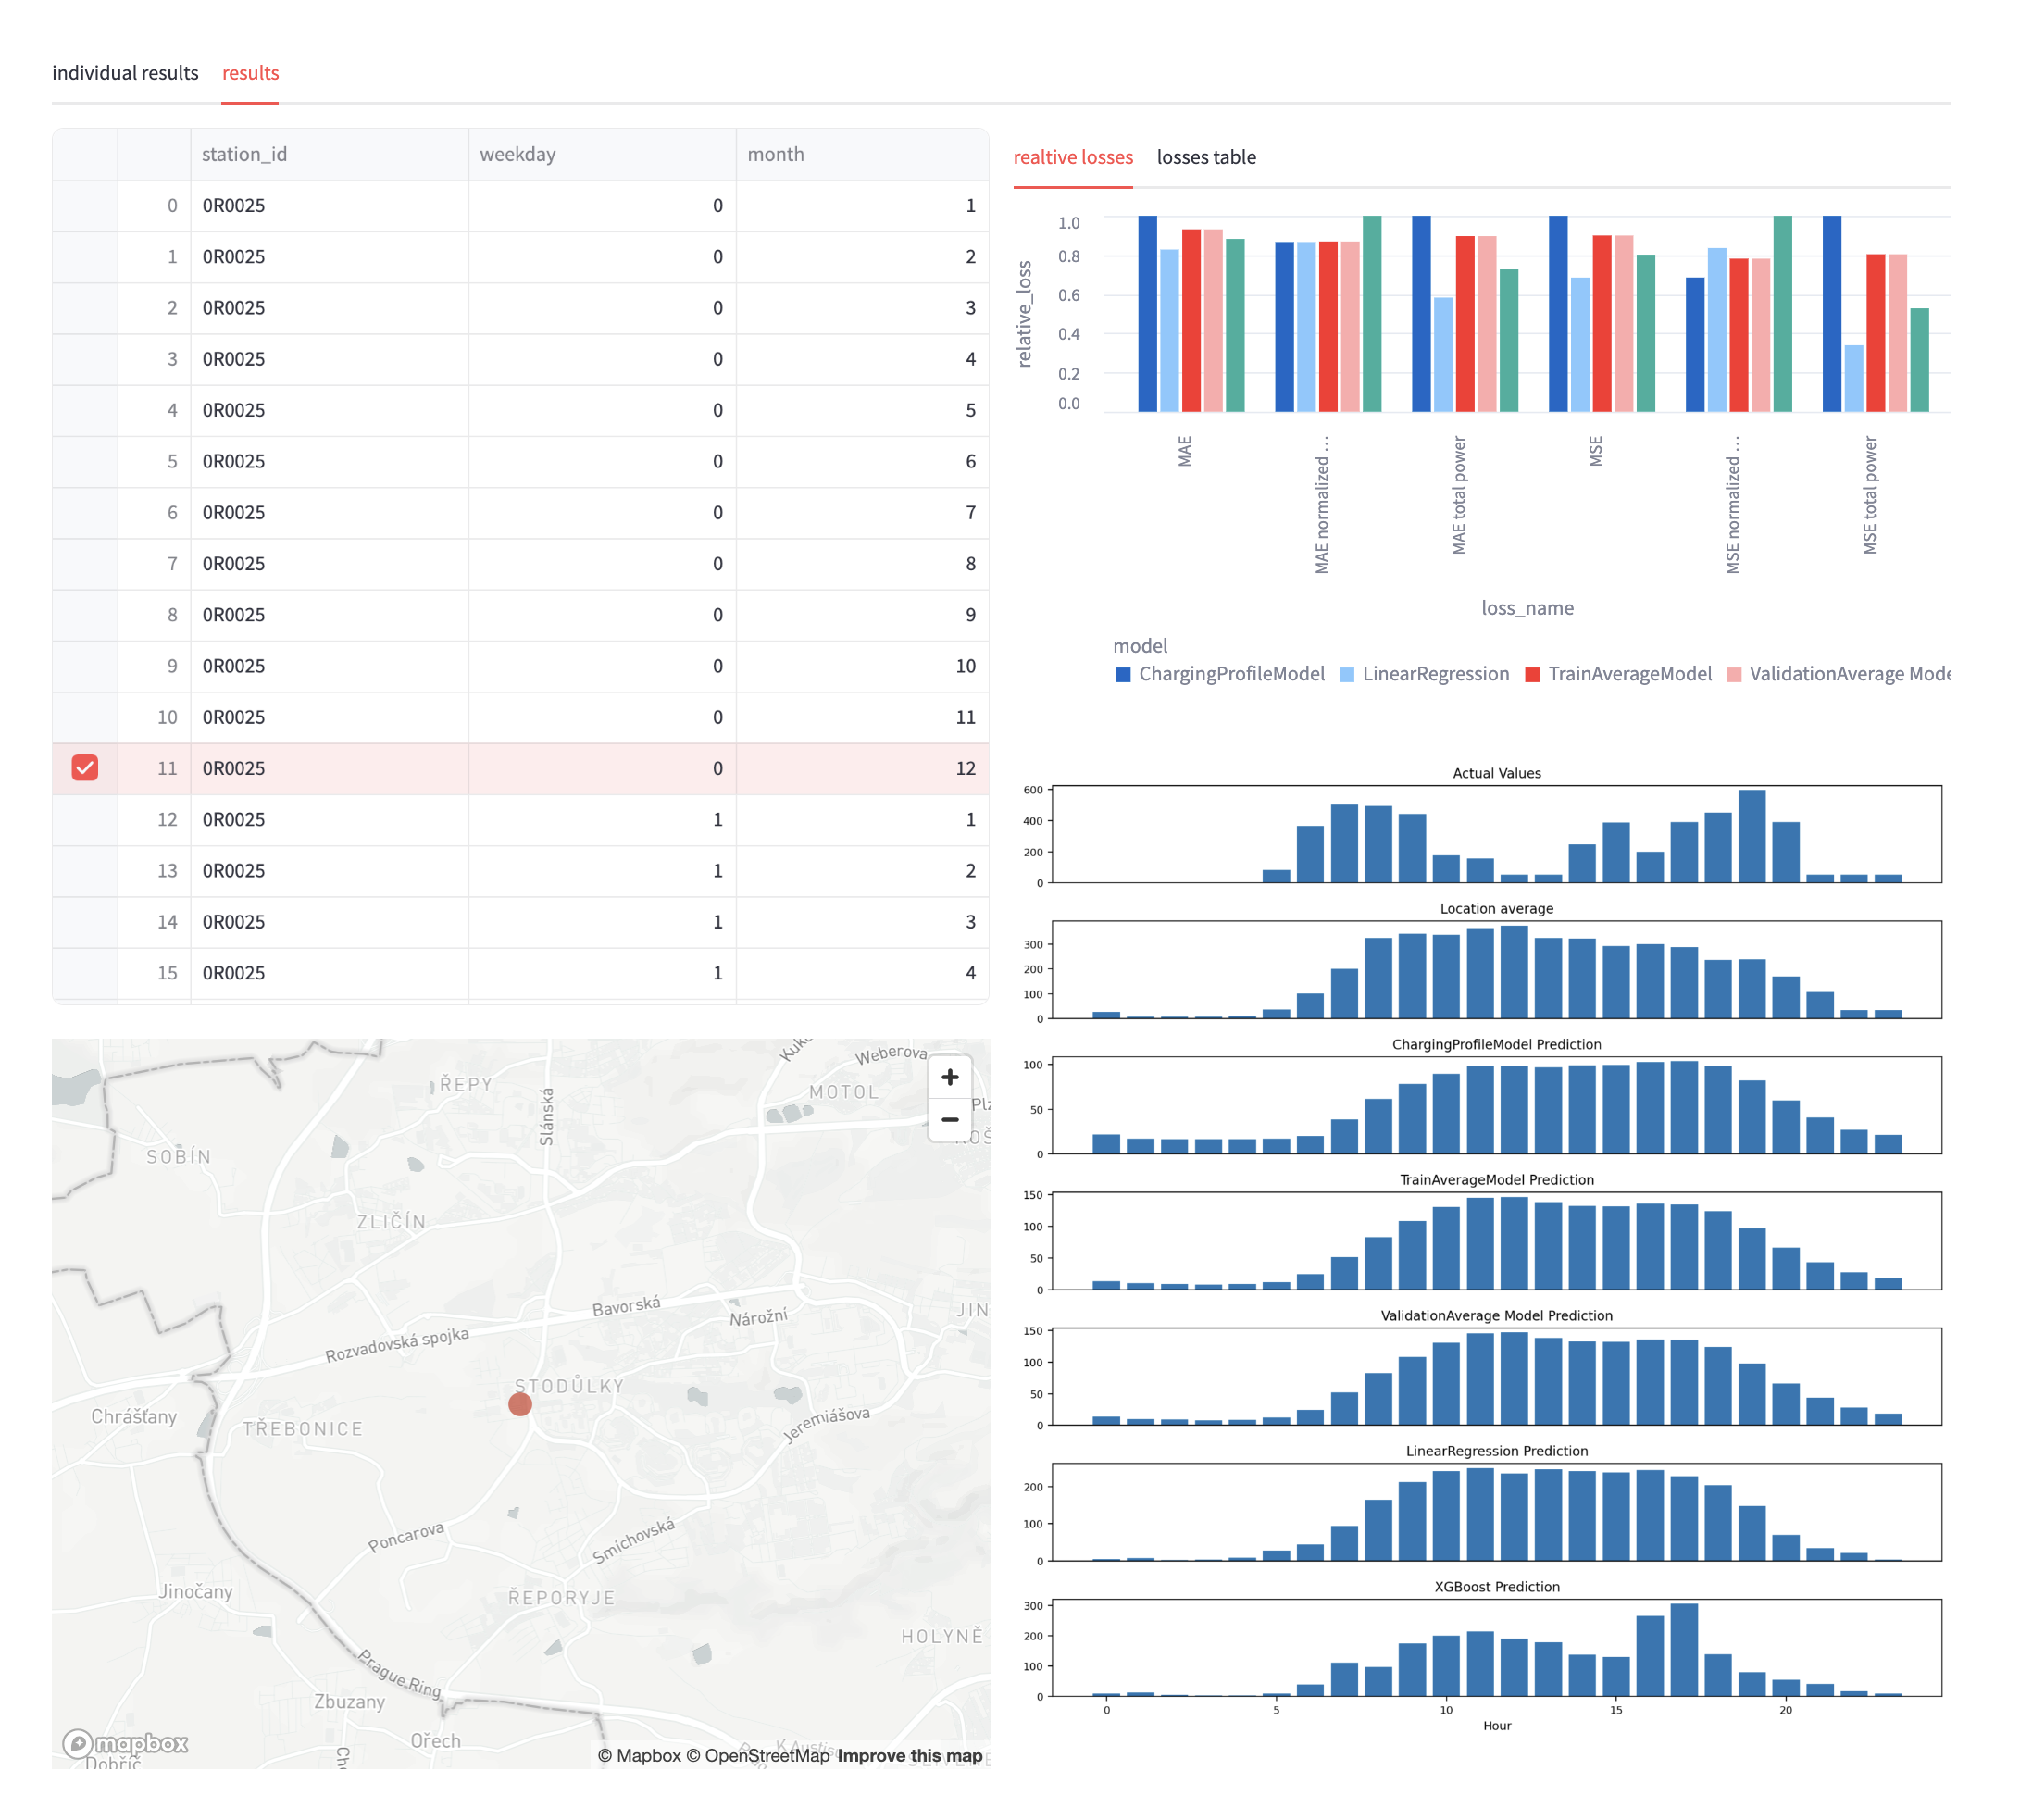
\includegraphics{data-dashboard-individual-predictions.png}
    \caption[]{Data dashboard website showing table with data from validation data set with one selected row. Of which the prediction is computed from the main model and the other models for comparison.}
    \labfig{dasboard-individual}
\end{figure}
